% Created 2023-09-05 Tue 17:03
% Intended LaTeX compiler: pdflatex
\documentclass[11pt]{article}
\usepackage[utf8]{inputenc}
\usepackage[T1]{fontenc}
\usepackage{graphicx}
\usepackage{longtable}
\usepackage{wrapfig}
\usepackage{rotating}
\usepackage[normalem]{ulem}
\usepackage{amsmath}
\usepackage{amssymb}
\usepackage{capt-of}
\usepackage{hyperref}
\author{bailun}
\date{\today}
\title{工厂方法}
\hypersetup{
 pdfauthor={bailun},
 pdftitle={工厂方法},
 pdfkeywords={},
 pdfsubject={},
 pdfcreator={Emacs 28.2 (Org mode 9.5.5)}, 
 pdflang={English}}
\begin{document}

\maketitle
\tableofcontents


\section{简单工厂(Simple Factory)}
\label{sec:orgc9c0e8e}

\subsection{UML}
\label{sec:orgc036f9c}
\begin{center}
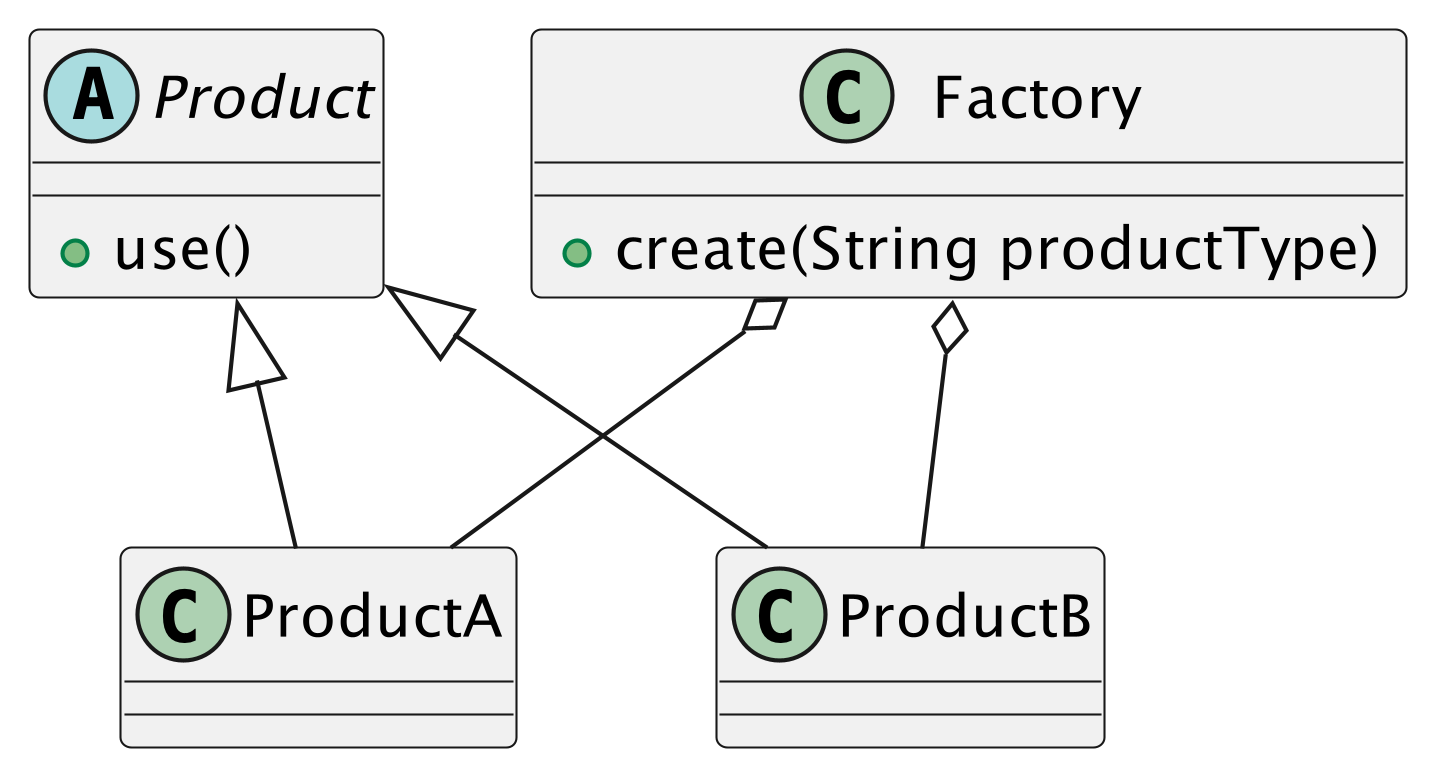
\includegraphics[width=.9\linewidth]{imgs/simple_factory.png}
\end{center}

\subsection{代码实现}
\label{sec:orgae2986c}

\begin{verbatim}
public class Excemple {
    public static abstract class Product {
	public abstract void use();
    }

    public static class ProductA extends Product {
	@Override
	public void use() {
	    System.out.println("Use Product A");
	}
    }

    public static class ProductB extends Product {
	@Override
	public void use() {
	    System.out.println("Use Product B");
	}
    }

    public static class Factory {
	public static Product create(String productName) {
	    if ("A".equals(productName)) {
		return new ProductA();
	    } else if ("B".equals(productName)) {
		return new ProductB();
	    }
	    return null;
	}
    }

    public static void main(String[] args) {
	Product productA = Factory.create("A");
	Product productB = Factory.create("B");
	productA.use();
	productB.use();
    }
}
\end{verbatim}
\end{document}